\documentclass{math}

\usepackage{enumerate}
\usepackage{tikz}

\geometry{letterpaper, margin=0.5in}

\title{Introduction to Intelligent Systems: Exam 3}
\author{Alvin Lin}
\date{August 2017 - December 2017}

\begin{document}

\maketitle

\subsection*{Problem 1}
Consider the following Bayesian Belief Network.
\begin{center}
  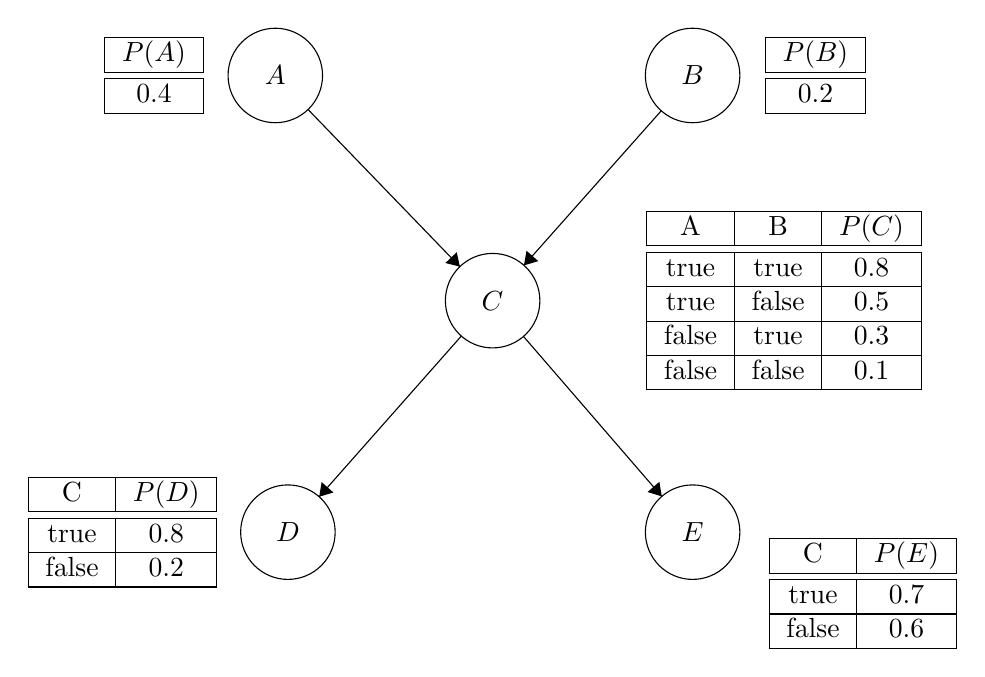
\begin{tikzpicture}[scale=0.2]
    \tikzstyle{every node}+=[inner sep=0pt]
    \draw [black] (31.5,-21.4) circle (3);
    \draw (31.5,-21.4) node {\( C \)};
    \draw (50, -21.4) node {
      \begin{tabular}{|c|c|c|}
        \hline
        A & B & \( P(C) \) \\ \hline \hline
        true & true & 0.8 \\ \hline
        true & false & 0.5 \\ \hline
        false & true & 0.3 \\ \hline
        false & false & 0.1 \\ \hline
      \end{tabular}
    };
    \draw [black] (18.5,-36.1) circle (3);
    \draw (18.5,-36.1) node {\( D \)};
    \draw (8, -36.1) node {
      \begin{tabular}{|c|c|}
        \hline
        C & \( P(D) \) \\ \hline \hline
        true & 0.8 \\ \hline
        false & 0.2 \\ \hline
      \end{tabular}
    };
    \draw [black] (44.2,-36.1) circle (3);
    \draw (44.2,-36.1) node {\( E \)};
    \draw (55, -40) node {
      \begin{tabular}{|c|c|}
        \hline
        C & \( P(E) \) \\ \hline \hline
        true & 0.7 \\ \hline
        false & 0.6 \\ \hline
      \end{tabular}
    };
    \draw [black] (17.7,-7.1) circle (3);
    \draw (17.7,-7.1) node {\( A \)};
    \draw (10, -7.1) node {
      \begin{tabular}{|c|}
      	\hline
    		\( P(A) \) \\ \hline \hline
    		0.4 \\ \hline
    	\end{tabular}
    };
    \draw [black] (44.2,-7.1) circle (3);
    \draw (44.2,-7.1) node {\( B \)};
    \draw (52, -7.1) node {
      \begin{tabular}{|c|}
      	\hline
    		\( P(B) \) \\ \hline \hline
    		0.2 \\ \hline
    	\end{tabular}
    };
    \draw [black] (29.51,-23.65) -- (20.49,-33.85);
    \fill [black] (20.49,-33.85) -- (21.39,-33.58) -- (20.64,-32.92);
    \draw [black] (19.78,-9.26) -- (29.42,-19.24);
    \fill [black] (29.42,-19.24) -- (29.22,-18.32) -- (28.5,-19.01);
    \draw [black] (42.21,-9.34) -- (33.49,-19.16);
    \fill [black] (33.49,-19.16) -- (34.4,-18.89) -- (33.65,-18.23);
    \draw [black] (33.46,-23.67) -- (42.24,-33.83);
    \fill [black] (42.24,-33.83) -- (42.09,-32.9) -- (41.34,-33.55);
  \end{tikzpicture}
\end{center}
\begin{enumerate}[(a)]
  \item Calculuate the initial probability of \( C \) given the data in the
  table.
  \begin{align*}
    P(C) &= P(C|A,B)\times P(A)\times P(B)+ \\
    & P(C|A,\neg B)\times P(A) \times P(\neg B)+ \\
    & P(C|\neg A,B)\times P(\neg A)\times P(B)+ \\
    & P(C|\neg A, \neg B)\times P(\neg A)\times P(\neg B) \\
    &= (0.8\times0.4\times0.2)+ \\
    & (0.5\times0.4\times(1-0.2))+ \\
    & (0.3\times(1-0.4)\times0.2)+ \\
    & (0.1\times(1-0.4)\times(1-0.2)) \\
    &= 0.064+0.16+0.036+0.048 \\
    &= 0.308
  \end{align*}
  \item Calculate \( P(A,B,\neg C,\neg D,E) \)
  \begin{align*}
    P(A,B,\neg C,\neg D,E) &= P(A)\times P(B)\times P(\neg C|A,B)\times
      P(\neg D|\neg C)\times P(E|\neg C) \\
    &= 0.4\times0.2\times(1-0.8)\times(1-0.2)\times0.6 \\
    &= 0.00768
  \end{align*}
\end{enumerate}

\subsection*{Decision Tree/Shannon Entropy}
Consider the following table for the Restaurant problem previous discussed:
\begin{center}
 \begin{tabular}{|c|c|c|c|c|c|c|c|c|c|c||c|}
    \hline
    Num & Alt & Bar & Fri & Hun & Pat & Price & Rain & Res & Type & Est &
      Wait \\ \hline \hline
    \( x_{1} \) & yes & no & no & yes & some & \$\$\$ & no & yes & French &
      0-10 & yes \\ \hline
    \( x_{2} \) & yes & no & no & yes & full & \$ & no & no & Thai & 30-60 &
      no \\ \hline
    \( x_{3} \) & no & yes & no & no & some & \$ & no & no & Burger & 0-10 &
      yes \\ \hline
    \( x_{4} \) & yes & no & yes & yes & full & \$ & yes & no & Thai & 10-30 &
      yes \\ \hline \hline
    \( x_{5} \) & yes & no & yes & no & full & \$\$\$ & no & yes & French &
      $>$60 & no \\ \hline
    \( x_{6} \) & no & yes & no & yes & some & \$\$ & yes & yes & Italian &
      0-10 & yes \\ \hline
    \( x_{7} \) & no & yes & no & no & none & \$ & yes & no & Burger & 0-10 &
      no \\ \hline
    \( x_{8} \) & no & no & no & yes & some & \$\$ & yes & yes & Thai & 0-10 &
      yes \\ \hline \hline
    \( x_{9} \) & no & yes & yes & no & full & \$ & yes & no & Burger & $>$60 &
      no \\ \hline
    \( x_{10} \) & yes & yes & yes & yes & full & \$\$\$ & no & yes & Italian &
      10-30 & no \\ \hline
    \( x_{11} \) & no & no & no & no & none & \$ & no & no & Thai & 0-10 &
      no \\ \hline
    \( x_{12} \) & yes & yes & yes & yes & full & \$ & no & no & Burger &
      30-60 & yes \\ \hline
  \end{tabular}
\end{center}
Using the Shannon Entropy formula and our formula for \textit{Gain}, calculate
the amount of information obtained by choosing the attribute of \textit{Price}.
\begin{align*}
  Gain(Price) &= B(\frac{6}{12})-\bigg[\frac{7}{12}B(\frac{3}{7})+
    \frac{2}{12}B(\frac{2}{2})+\frac{3}{12}B(\frac{1}{3})\bigg] \\
  &= 1-\bigg[\frac{7}{12}\times0.985+0+\frac{3}{12}\times0.918\bigg] \\
  &= 1-\bigg[0.804\bigg] \\
  &= 0.196~\text{bits}
\end{align*}

\begin{center}
  If you have any questions, comments, or concerns, please contact me at
  alvin@omgimanerd.tech
\end{center}

\end{document}
